\section{Generative Adversarial Networks}
\subsection*{Density Estimation}
Gen.M:$p(x)$, para.M: $p_{\theta}(x)$, Goal: $p_{\theta}(x)=p(x)$.

But:Colps:$p(x)>>p_{\theta}(x)\stackrel{>}{\approx}0$, bad $\mathcal{D}$: $p(x)>>p_{\theta}(x)\stackrel{>}{\approx}0$, norm./integr. (-> EM). MLE:$\hat{\theta}=\text{amax}_{\theta} \mathbb{E}_{x\sim p}[\ln p_{\theta}(x)]\approx \text{amax}_{\theta} \frac{1}{L}\sum\ln p_{\theta}(x)$

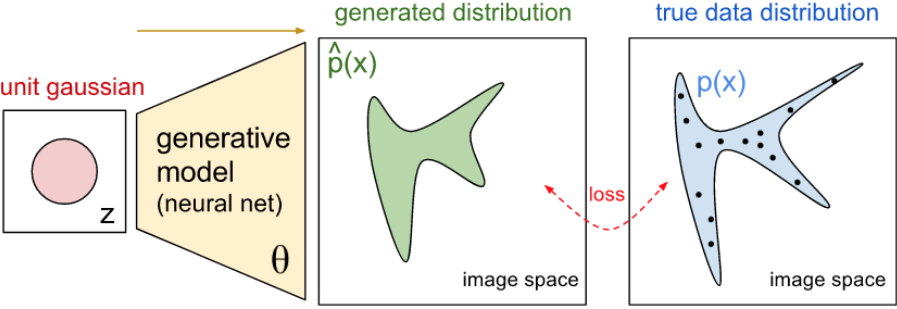
\includegraphics[width=\textwidth/6]{ETH-DS-2020/AML/Resources/gans.png}

$z\sim f$ (rand), $x=NN_{\theta}(z)$ (det)

Likelihood based GANs: opt $\log p(x)$ 

\subsection*{GANs (1. Generate, 2. Classify: Real 1/Fake 0)}
G.f.'14: 
1.$\tilde{p}_{\theta}(x,y)=\frac{1}{2}(y p(x)+(1-y)p_{\theta}(x))$

2.BayesOptClas: $q_{\theta}(x)=\frac{p(x)}{p(x)+p_{\theta}(x)}=P(y=1|x)$

3.$l^*(\theta)= \E_{\tilde{p}_{\theta}}[y\ln q_{\theta}(x)+(1-y)\ln(1-q_{\theta})]$

4. BOC=?, so $q_{\theta}\rightarrow q_{\phi}$ \& $l^*(\theta)\rightarrow \sup_{\phi} l(\theta,\phi)$:

$l^*(\theta)\ge\sup_{\phi}\E_{\tilde{p}_{\theta}}[y\ln q_{\phi}(x)+(1-y)\ln(1-q_{\phi}(x))]$

5.Sadl:$\argmin\{\sup_{\phi} l(\theta,\phi)\}$, so SGD may $\rightarrow \infty$

$(\theta,\phi)^{t+1}=(\theta,\phi)^t+\eta(- \nabla_{\theta} l(\theta^t,\phi^t), \nabla_{\theta}l(\theta^{t+1},\phi^t))$

$\min\limits_G\max\limits_D \E_{x\sim\mathcal{D}}\log D(x)+\E_{z\sim p_z}\log(1-D(G(z)))$

Chllng:Qual ctrl;Trd-of: noisy vs. mode drop

Gf. GAN '14 <DC GAN: Radford '15 < Prog.-Grow. GAN: NVIDIA '18 < CycleGAN

COV (w $f_{\theta}=g_{\theta}^{-1}$): $p_X(x)=p_Z(f(x))|\det (\frac{\partial f_{\theta}(x)}{\partial x^T})|$

Opt: $\min_{\theta}\E[-\log(p_{\theta}(x))]$;
\term{Normalizing flows:} bij. $F$ s.t. eval, invert and $|\det(\partial F)|$ easy 

$F^{-1}=F_1^{-1}\circ\cdots\circ F_L^{-1}$, $\det (\partial F)=\prod^1_{l=L}\det(\partial F_l\circ F_{l-1:1})$, $\det(\partial F^{-1})=\det(\partial F)^{-1}$

Log-likelihood: $ p_X(x) = \text{log}(p_Z(F(\mathbf{x})))  - \sum^L_{l=1}\log|\det(\partial F_l\circ F_{1:l-1})|$

SimpTrafo: $y_{d+1  :D}=x_{d+1:D}\odot\exp s(x_{1:d})+t(x_{1:d})$

%\textcolor{red}{Not sure what to add about "factoring out" and "Glow" etc, slides 31+}